% --- TÓM TẮT BÁO CÁO ---
\section*{TÓM TẮT BÁO CÁO (ABSTRACT)}
Nghiên cứu này đề xuất và đánh giá một hệ thống Multi-Agent Mô hình Ngôn ngữ Lớn (LLM) tích hợp Truy hồi thông tin kết hợp (Hybrid Retrieval-Augmented Generation - RAG) và Bộ nhớ đa tầng (Short-term \& Long-term Memory) nhằm nâng cao độ chính xác thực chứng (factual accuracy) trong giải quyết các câu hỏi y khoa phức tạp thuộc bộ dữ liệu benchmark MedQA-USMLE (1.273 câu hỏi kiểm thử chính thức). Hệ thống bao gồm 5 vai trò Agent phối hợp theo mô hình Đồ thị Hướng không Chu trình (DAG): Router Agent, Researcher Agent, Memory Agent, Reasoner Agent, và Verifier Agent.

Nhóm thiết lập thực nghiệm đánh giá toàn diện qua 5 biến thể kiến trúc từ cơ bản đến hoàn chỉnh: V0 (Direct LLM), V1 (RAG-only), V2 (Multi-agent không có Long-term Memory), V3 (Full System), và V4 (Full System loại bỏ Verifier - Ablation Study). Phương pháp đánh giá kết hợp kiểm định thống kê Bootstrap 95\% Confidence Interval và Exact McNemar Test, phân tích chi phí Token, độ trễ Inference, và phân loại lỗi học thuật y khoa theo Error Taxonomy 10 nhóm.

Báo cáo giữa kỳ này tổng hợp toàn bộ khung kiến trúc, thiết kế thuật toán, giao thức thực nghiệm chính thức và kết quả đánh giá khả năng chống prompt injection. Thí nghiệm bổ sung chạy theo cặp clean/attacked trên toàn bộ 1.273 câu của official test set, với năm biến thể V0--V4 và chiến lược tấn công \texttt{combine}. Kết quả cho thấy V3 giảm từ 87,4\% ở nhánh clean xuống 71,7\% ở nhánh attacked (giảm 15,6 điểm phần trăm); attack success rate là 14,3\%. V4 có mức giảm lớn nhất (16,7 điểm phần trăm) và ASR cao nhất (22,1\%).

Thí nghiệm defense với \texttt{semantic\_guard} cho thấy attacked accuracy
được khôi phục bằng clean accuracy ở cả năm variant; accuracy drop,
conditional ASR và prediction flip rate đều bằng 0\% trên toàn bộ 1.273 câu.

\vspace{0.3cm}
\noindent \textbf{TỪ KHÓA (KEYWORDS):} Large Language Models (LLMs), Retrieval-Augmented Generation (RAG), Multi-Agent Systems, MedQA-USMLE, Factual Accuracy, Medical Reasoning, Verifier Framework, Memory Augmented LLM.

\vspace{0.5cm}

% --- DANH MỤC TỪ VIẾT TẮT ---
\section*{DANH MỤC TỪ VIẾT TẮT (GLOSSARY)}
\begin{table}[h!]
\centering
\begin{tabular}{lll}
\toprule
\textbf{Từ viết tắt} & \textbf{Tên đầy đủ bằng tiếng Anh} & \textbf{Nghĩa tiếng Việt} \\
\midrule
LLM & Large Language Model & Mô hình ngôn ngữ lớn \\
RAG & Retrieval-Augmented Generation & Sinh văn bản tăng cường truy hồi \\
DAG & Directed Acyclic Graph & Đồ thị hướng không chu trình \\
USMLE & United States Medical Licensing Examination & Kỳ thi cấp phép hành nghề y khoa Hoa Kỳ \\
BM25 & Best Matching 25 & Thuật toán truy hồi văn bản dựa trên tần suất từ \\
MMR & Maximal Marginal Relevance & Thuật toán đa dạng hóa kết quả truy hồi \\
CI & Confidence Interval & Khoảng tin cậy \\
JSONL & JSON Lines & Định dạng dữ liệu ghi nhận câu hỏi/kết quả \\
\bottomrule
\end{tabular}
\end{table}

\newpage

% --- 1. INTRODUCTION ---
\section{INTRODUCTION}

\subsection{Bối cảnh}
Trong những năm gần đây, Mô hình Ngôn ngữ Lớn (LLM) đã đạt được những tiến bộ vượt bậc trong xử lý ngôn ngữ tự nhiên và lập luận tổng quát. Tuy nhiên, việc áp dụng LLM vào lĩnh vực y tế đòi hỏi độ chính xác tuyệt đối về mặt thực chứng (factual accuracy). Hiện tượng ảo giác (hallucination), lập luận y khoa sai lệch hoặc bỏ sót các chi tiết lâm sàng quan trọng vẫn là những rào cản lớn khi ứng dụng LLM trong tri thức y khoa.

\subsection{Vấn đề nghiên cứu}
Bộ câu hỏi MedQA-USMLE mô phỏng kỳ thi cấp phép hành nghề y khoa Hoa Kỳ, đòi hỏi mô hình không chỉ ghi nhớ tri thức sinh học/y khoa thuần túy mà phải có khả năng suy luận lâm sàng đa bước (multi-step clinical reasoning), kết hợp các triệu chứng, xét nghiệm, yếu tố dịch tễ để đưa ra đáp án chính xác. Các mô hình sinh văn bản đơn lẻ (Zero-shot / Direct Prompting) thường gặp hạn chế do dung lượng ngữ cảnh, khả năng tự kiểm định kém và thiếu cơ chế truy hồi tri thức chuẩn xác.

\subsection{Mục tiêu}
Xây dựng, tối ưu hóa và đánh giá thực nghiệm một hệ thống Multi-Agent LLM tích hợp Hybrid RAG và Long-term Memory nhằm tối đa hóa độ chính xác thực chứng trên tập kiểm thử MedQA-USMLE.

\textit{Lưu ý phạm vi:} Đề tài tập trung thuần túy vào mặt thiết kế hệ thống, phương pháp luận AI và đánh giá benchmark thực nghiệm; không nhằm mục đích triển khai hỗ trợ chẩn đoán lâm sàng trực tiếp trên bệnh nhân thực tế.

\subsection{Đóng góp của đề tài}
\begin{itemize}
    \item Đề xuất kiến trúc Multi-Agent phối hợp 5 vai trò chuyên biệt xử lý bài toán MedQA-USMLE dưới dạng khung thực thi DAG.
    \item Cung cấp quy trình Hybrid RAG tối ưu hóa chuyên biệt cho thuật ngữ y học (kết hợp Dense Vector Search \& Sparse BM25).
    \item Xây dựng giao thức kiểm thử chính thức (Official Evaluation Protocol) ngặt nghèo, đảm bảo tính đóng băng cấu hình (freeze) và chống rò rỉ dữ liệu (data leakage).
    \item Cung cấp mã nguồn mở hoàn chỉnh (\texttt{medqa-multiagent}) tích hợp bộ công cụ CLI và giao diện Streamlit tương tác.
\end{itemize}

\section{SYSTEM ARCHITECTURE}

\subsection{Kiến trúc tổng quan}
Hệ thống được thiết kế theo mô hình Multi-Agent hướng sự kiện và đồ thị tác vụ. Các Agent đóng vai trò là các nút (nodes) trong hệ thống, trao đổi trạng thái nội bộ thông qua một bộ nhớ ngắn hạn (Short-term Memory State).

% Thêm vào preamble nếu chưa có:
% \usepackage{tikz}
% \usepackage{graphicx}
% \usetikzlibrary{arrows.meta}

\begin{figure}[h!]
\centering

\resizebox{0.96\textwidth}{!}{%
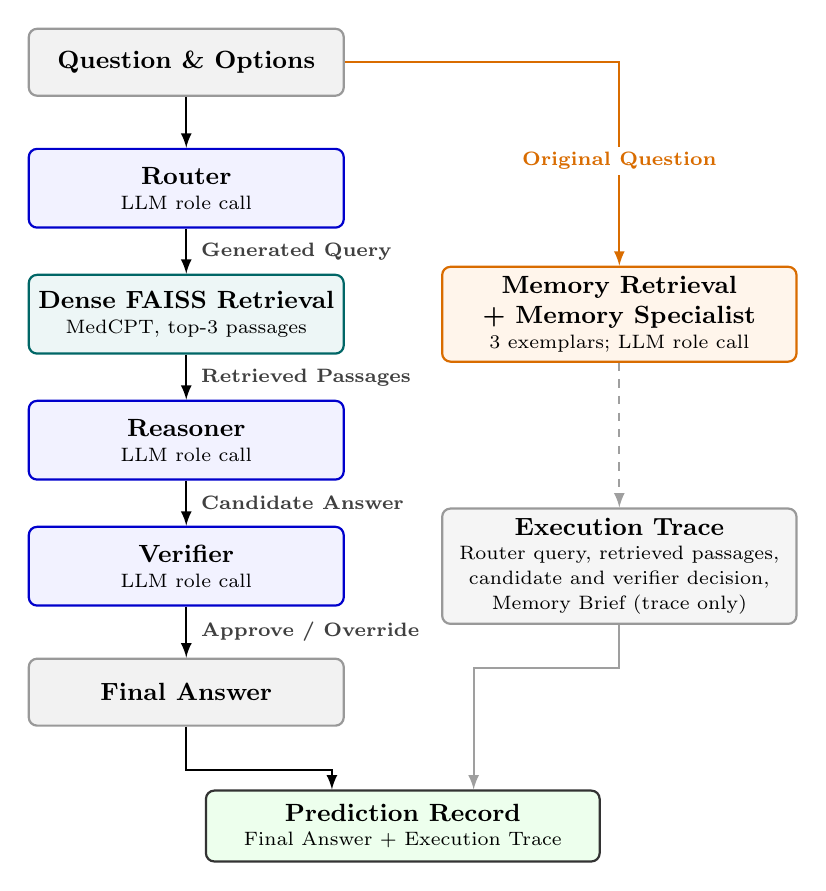
\begin{tikzpicture}[
    >=latex,
    font=\small,
    agent/.style={
        draw=blue!80!black,
        fill=blue!5,
        rectangle,
        rounded corners=3pt,
        minimum width=4cm,
        minimum height=1cm,
        align=center,
        thick
    },
    retrieval/.style={
        draw=teal!80!black,
        fill=teal!7,
        rectangle,
        rounded corners=3pt,
        minimum width=4cm,
        minimum height=1cm,
        align=center,
        thick
    },
    memory/.style={
        draw=orange!85!black,
        fill=orange!8,
        rectangle,
        rounded corners=3pt,
        minimum width=4.5cm,
        minimum height=1.15cm,
        align=center,
        thick
    },
    trace/.style={
        draw=gray!80,
        fill=gray!8,
        rectangle,
        rounded corners=3pt,
        minimum width=4.5cm,
        minimum height=1.4cm,
        align=center,
        thick
    },
    io/.style={
        draw=gray!80,
        fill=gray!10,
        rectangle,
        rounded corners=3pt,
        minimum width=4cm,
        minimum height=0.85cm,
        align=center,
        thick
    },
    record/.style={
        draw=black!80,
        fill=green!7,
        rectangle,
        rounded corners=3pt,
        minimum width=5cm,
        minimum height=0.9cm,
        align=center,
        thick
    },
    lbl/.style={
        font=\scriptsize\bfseries,
        text=black!75,
        fill=white,
        inner sep=2pt
    }
]

\node[io] (question) at (0,0)
    {\textbf{Question \& Options}};

\node[agent] (router) at (0,-1.6)
    {\textbf{Router}\\[-2pt]
     \scriptsize LLM role call};

\node[retrieval] (rag) at (0,-3.2)
    {\textbf{Dense FAISS Retrieval}\\[-2pt]
     \scriptsize MedCPT, top-3 passages};

\node[agent] (reasoner) at (0,-4.8)
    {\textbf{Reasoner}\\[-2pt]
     \scriptsize LLM role call};

\node[agent] (verifier) at (0,-6.4)
    {\textbf{Verifier}\\[-2pt]
     \scriptsize LLM role call};

\node[io] (answer) at (0,-8.0)
    {\textbf{Final Answer}};


\node[memory] (memory) at (5.5,-3.2)
    {\textbf{Memory Retrieval}\\
     \textbf{+ Memory Specialist}\\[-2pt]
     \scriptsize 3 exemplars; LLM role call};

\node[trace] (trace) at (5.5,-6.4)
    {\textbf{Execution Trace}\\[-2pt]
     \scriptsize Router query, retrieved passages,\\[-2pt]
     \scriptsize candidate and verifier decision,\\[-2pt]
     \scriptsize Memory Brief (trace only)};


\node[record] (record) at (2.75,-9.7)
    {\textbf{Prediction Record}\\[-2pt]
     \scriptsize Final Answer + Execution Trace};


\draw[->, thick]
    (question) --
    (router);

\draw[->, thick]
    (router) --
    node[lbl, right=3pt] {Generated Query}
    (rag);

\draw[->, thick]
    (rag) --
    node[lbl, right=3pt] {Retrieved Passages}
    (reasoner);

\draw[->, thick]
    (reasoner) --
    node[lbl, right=3pt] {Candidate Answer}
    (verifier);

\draw[->, thick]
    (verifier) --
    node[lbl, right=3pt] {Approve / Override}
    (answer);

\draw[->, thick, orange!85!black]
    (question.east) --
    ++(1.0,0) -|
    (memory.north);

\node[
    lbl,
    text=orange!85!black
] at (5.5,-1.25)
    {Original Question};

\draw[
    ->,
    thick,
    dashed,
    gray!75
]
    (memory.south) --
    (trace.north);


\draw[->, thick]
    (answer.south) --
    ++(0,-0.55) -|
    ([xshift=-0.9cm]record.north);

\draw[->, thick, gray!75]
    (trace.south) --
    ++(0,-0.55) -|
    ([xshift=0.9cm]record.north);

\end{tikzpicture}%
}

\caption{Kiến trúc tổng thể hệ thống MEDQA MULTI-AGENT}
\label{fig:v3_actual_pipeline}

\end{figure}

\subsection{Luồng xử lý}
\begin{enumerate}
    \item \textbf{Input:} Câu hỏi lâm sàng MedQA và 4/5 lựa chọn đáp án.
    \item \textbf{Routing:} Router Agent trích xuất từ khóa, bệnh lý chính, tạo câu truy vấn RAG và câu truy vấn tìm ca bệnh tương tự.
    \item \textbf{Retrieval \& Memory Synthesis:}
    \begin{itemize}
        \item Researcher Agent thực thi Hybrid Search thu thập các passage y khoa.
        \item Memory Agent truy vấn cơ sở dữ liệu các ca bệnh đã giải trước đó.
    \end{itemize}
    \item \textbf{Reasoning:} Reasoner Agent tổng hợp thông tin, tiến hành loại trừ đáp án sai và đề xuất đáp án ứng viên.
    \item \textbf{Verification:} Verifier Agent đối chiếu lập luận của Reasoner với bằng chứng RAG. Nếu phát hiện mâu thuẫn, Verifier phát ra feedback để Reasoner lập luận lại hoặc tiến hành Override đáp án.
\end{enumerate}

\subsection{Các biến thể V0--V4}

Để đánh giá tác động của từng thành phần, hệ thống định nghĩa năm
biến thể V0--V4 như trình bày trong Bảng~\ref{tab:variants}.

\begin{table}[H]
\centering
\caption{So sánh các thành phần được sử dụng trong V0--V4.}
\label{tab:variants}

\resizebox{\textwidth}{!}{%
\begin{tabular}{lccccc}
\toprule
\textbf{Variant}
& \textbf{\shortstack{Direct\\Answering}}
& \textbf{\shortstack{RAG\\Retrieval}}
& \textbf{\shortstack{Multi-Agent\\Workflow}}
& \textbf{\shortstack{Long-term\\Memory}}
& \textbf{\shortstack{Verifier\\Role}} \\
\midrule
V0 & Có    & Không & Không & Không & Không \\
V1 & Có    & Có    & Không & Không & Không \\
V2 & Không & Có    & Có    & Không & Có    \\
V3 & Không & Có    & Có    & Có*   & Có    \\
V4 & Không & Có    & Có    & Có    & Không \\
\bottomrule
\end{tabular}%
}

\vspace{2mm}

\begin{minipage}{0.96\textwidth}
\footnotesize
\textit{Ghi chú:} Trong V3, Memory Specialist tạo
\texttt{memory\_brief} và lưu nó trong prediction trace, nhưng nội
dung này chưa được truyền vào Reasoner. Do đó, ký hiệu ``Có*''
không đồng nghĩa Long-term Memory đã tác động đến đáp án cuối.
\end{minipage}

\end{table}

% Không cho bảng trôi qua subsection tiếp theo
\FloatBarrier

% Nếu không còn đủ chỗ cho subsection và listing,
% tự động chuyển cả phần xuống trang mới
\Needspace{14\baselineskip}

\subsection{Giao diện Black-Box Entrypoint}

Mọi biến thể được gọi thông qua cùng một hàm entrypoint. Tham số
\texttt{variant} quyết định luồng xử lý nội bộ, trong khi kiểu dữ
liệu đầu vào và đầu ra được giữ thống nhất.

\begin{lstlisting}[
    language=Python,
    basicstyle=\ttfamily\footnotesize,
    breaklines=true,
    columns=fullflexible,
    keepspaces=true,
    frame=single
]
def answer_question(
    question: str,
    options: Mapping[str, str],
    variant: str,
    config: RunConfig,
    client: LLMClient,
    retriever: Optional[Retriever] = None,
    user_id: str = "default_user",
) -> AnswerResult:
    ...
\end{lstlisting}

\Needspace{9\baselineskip}

\subsection{Prediction Trace và Reproducibility}

Mỗi dự đoán được lưu thành một JSON object trong file JSONL. Một
prediction record bao gồm mã câu hỏi, biến thể, đáp án dự đoán, đáp
án chuẩn, trạng thái đúng/sai, trạng thái đầu ra không hợp lệ, phần
giải thích, tổng số prompt token, completion token, total token,
tổng latency và trường \texttt{trace}.

Nội dung \texttt{trace} phụ thuộc vào từng biến thể. V0 có trace
rỗng; V1 lưu các passage được truy hồi; V2 và V3 lưu thêm truy vấn
của Router, candidate answer của Reasoner và quyết định của
Verifier. V3 còn lưu \texttt{memory\_brief}, trong khi V4 lưu
\texttt{research\_brief}, \texttt{memory\_brief} và trạng thái
\texttt{verifier\_omitted}.

Các prompt đầy đủ được ghi nhận bởi lớp logging của LLM client,
nhưng không nằm trực tiếp trong prediction JSONL. Prediction trace
chỉ lưu trạng thái trung gian và phần giải thích do mô hình cung
cấp; hệ thống không tuyên bố lưu toàn bộ chuỗi suy luận nội bộ của
mô hình.
% --- 3. SYSTEM DESIGN ---
\section{SYSTEM DESIGN}

\subsection{Agent Architecture}
\subsubsection{Router Agent}
\textbf{Nhiệm vụ:} Phân tích câu hỏi y khoa, trích xuất thực thể lâm sàng (triệu chứng, diễn tiến, xét nghiệm) và tạo truy vấn tìm kiếm RAG. Có khả năng tái cấu trúc truy vấn (reformulate) khi bằng chứng thu được chưa đạt chất lượng.

\subsubsection{Researcher Agent}
\textbf{Nhiệm vụ:} Nhận truy vấn từ Router, thực hiện Hybrid Retrieval trên ngữ cảnh y học, loại bỏ thông tin nhiễu và tổng hợp thành Research Brief ngắn gọn.

\subsubsection{Memory Agent}
\textbf{Nhiệm vụ:} Tìm kiếm các ví dụ ca bệnh có đặc điểm triệu chứng tương đồng trong cơ sở dữ liệu Long-term Memory, tổng hợp thành Memory Brief nhằm hỗ trợ tri thức kinh nghiệm cho Reasoner.

\subsubsection{Reasoner Agent}
\textbf{Nhiệm vụ:} Thực hiện suy luận lâm sàng đa bước. Phân tích chẩn đoán phân biệt, loại trừ các phương án bất hợp lý, đưa ra Candidate Answer kèm lời giải thích ngắn (Explanation).

\subsubsection{Verifier Agent}
\textbf{Nhiệm vụ:} Kiểm định tính xác thực của Candidate Answer. Kiểm tra tính hợp lệ của phương án được chọn, đối chiếu câu chữ với Research Brief. Đưa ra quyết định: Approve (Đồng ý), Override (Ghi đè đáp án mới) hoặc Feedback (Yêu cầu Reasoner chạy lại).

\subsubsection{DAG Orchestration}
Hệ thống tích hợp một DAG Engine tự xây dựng bằng Python hỗ trợ phát hiện chu trình (cycle detection), sắp xếp thứ tự phụ thuộc (topological sort) và sử dụng \texttt{ThreadPoolExecutor} để chạy song song các Agent độc lập (như Researcher và Memory Agent).

\subsection{RAG Design}
\begin{itemize}
    \item \textbf{Corpus Loading \& Chunking:} Tài liệu y khoa được chia đoạn với kích thước chuẩn $chunk\_size = 256$ tokens.
    \item \textbf{Hybrid Retrieval:} Kết hợp tìm kiếm không gian Vector (Dense Embedding) và từ khóa kề cận (Sparse BM25).
    \item \textbf{Fusion \& Ranking:} Sử dụng Reciprocal Rank Fusion (RRF) để hợp nhất bảng xếp hạng kết quả từ BM25 và Vector Search, lấy ra Top-$k$ ($k=3$) đoạn văn bản liên quan nhất.
\end{itemize}

\begin{figure}[h!]
\centering
\resizebox{\textwidth}{!}{%
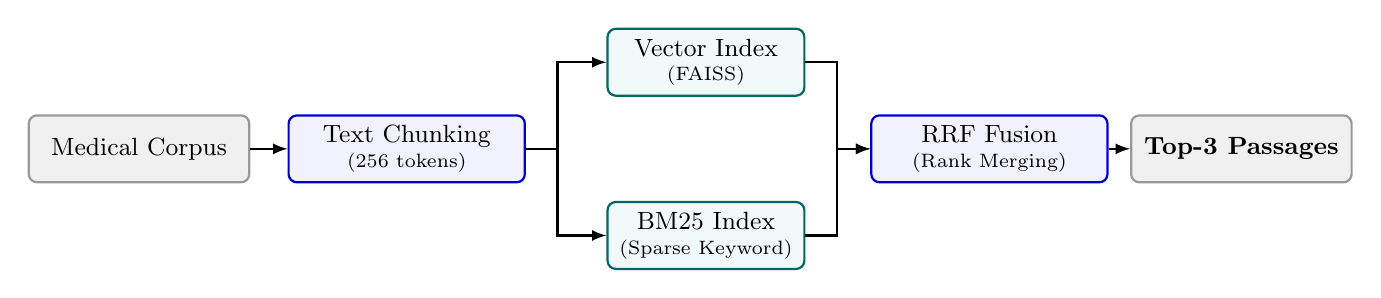
\begin{tikzpicture}[
    >=latex,
    font=\small,
    io/.style={draw=gray!80, fill=gray!12, rectangle, rounded corners=3pt, minimum width=2.8cm, minimum height=0.85cm, align=center, thick},
    block/.style={draw=blue!80!black, fill=blue!5, rectangle, rounded corners=3pt, minimum width=3.0cm, minimum height=0.85cm, align=center, thick},
    idx/.style={draw=teal!80!black, fill=teal!5, rectangle, rounded corners=3pt, minimum width=2.5cm, minimum height=0.85cm, align=center, thick}
]

    \node [io] (A) at (0, 0) {Medical Corpus};
    \node [block] (B) at (3.4, 0) {Text Chunking\\[-2pt]\scriptsize(256 tokens)};
    \node [idx] (C1) at (7.2, 1.1) {Vector Index\\[-2pt]\scriptsize(FAISS)};
    \node [idx] (C2) at (7.2, -1.1) {BM25 Index\\[-2pt]\scriptsize(Sparse Keyword)};
    \node [block] (D) at (10.8, 0) {RRF Fusion\\[-2pt]\scriptsize(Rank Merging)};
    \node [io] (E) at (14.0, 0) {\textbf{Top-3 Passages}};

    \draw [->, thick] (A) -- (B);
    \draw [->, thick] (B.east) -- ++(0.4, 0) |- (C1.west);
    \draw [->, thick] (B.east) -- ++(0.4, 0) |- (C2.west);
    \draw [->, thick] (C1.east) -| ++(0.4, -1.1) -- (D.west);
    \draw [->, thick] (C2.east) -| ++(0.4, 1.1) -- (D.west);
    \draw [->, thick] (D) -- (E);

\end{tikzpicture}%
}
\caption{Quy trình xử lý dữ liệu và truy hồi thông tin y khoa (RAG Pipeline).}
\label{fig:rag_pipeline}
\end{figure}

\subsection{Memory Design}
\begin{itemize}
    \item \textbf{Short-term Memory:} Tồn tại trong suốt chu trình xử lý một câu hỏi, chứa trạng thái trung gian của các Agent, được truyền liên tục qua DAG state.
    \item \textbf{Long-term Memory:} Lưu giữ các ca bệnh đã giải chính xác từ tập huấn luyện dưới dạng các bản ghi JSON (\texttt{case\_id}, \texttt{question}, \texttt{options}, \texttt{correct\_answer}, \texttt{explanation}). Sử dụng kỹ thuật truy hồi tương đồng từ khóa/ngữ nghĩa để lấy ra top-$k$ ca bệnh mẫu.
\end{itemize}

\textit{Hạn chế thực tế của Repository:} Hiện tại default long-term memory store mới chỉ chứa một số ca y khoa mẫu được soạn trước. Quy trình tự động xây dựng memory từ các dự đoán đúng trên tập Development, kiểm chứng, đóng băng (freeze) và đưa vào chạy Official Test vẫn đang trong quá trình hoàn thiện.

\subsection{Verifier Design}
Verifier Agent áp dụng bộ tiêu chí kiểm định nghiêm ngặt:
\begin{enumerate}
    \item Đáp án chọn có thuộc tập \{A, B, C, D\} hợp lệ không?
    \item Bằng chứng RAG thu thập được có ủng hộ trực tiếp hay bác bỏ đáp án ứng viên không?
    \item Lập luận của Reasoner có bị mâu thuẫn logic nội tại không?
\end{enumerate}

\subsection{Evolutionary Optimization}
Trong phạm vi hiện tại của repository, thành phần Evolutionary Optimization chưa được triển khai. Hệ thống chưa tích hợp thuật toán di truyền (Genetic Algorithm), đột biến prompt (Prompt Mutation) hay chọn lọc tự nhiên qua các thế hệ. Thành phần này được xếp vào hướng phát triển tương lai.

% --- 4. EXPERIMENTAL SETUP ---
\section{EXPERIMENTAL SETUP}

\subsection{Dataset}
Sử dụng bộ dữ liệu chuẩn MedQA-USMLE (tiếng Anh):
\begin{itemize}
    \item \textbf{Official Test set:} 1.273 câu
\end{itemize}

\subsection{Development Protocol}
Trích xuất ngẫu nhiên mẫu $N_{dev} = 100$ câu từ \texttt{data/dev.jsonl} với fixed seed = 42 để tinh chỉnh prompt, cấu hình RAG và kiểm tra luồng thực thi Agent.

\subsection{Official Evaluation Protocol}
Đóng băng toàn bộ cấu hình, prompt template và mã nguồn. Thực thi độc lập từng variant (V0-V4) trên toàn bộ $N_{test} = 1.273$ câu của \texttt{data/test.jsonl}. Kết quả được ghi nhận vào các file prediction riêng biệt: \texttt{predictions\_v0.jsonl} đến \texttt{predictions\_v4.jsonl}.

\subsection{Model and Prompts}
\begin{itemize}
    \item \textbf{Main Model:} deepseek-chat
    \item \textbf{Provider:} DeepSeek API, thông qua endpoint OpenAI-compatible: \texttt{https://api.deepseek.com/v1}
    \item \textbf{Temperature:} 0.0 (Đảm bảo tính xác định cao nhất).
    \item \textbf{Random seed:} 42
\end{itemize}

\subsection{Retrieval Configuration}
\begin{itemize}
    \item \textbf{Embedding model:}
    \begin{itemize}
        \item Query encoder: \texttt{ncbi/MedCPT-Query-Encoder}
        \item Passage encoder: \texttt{ncbi/MedCPT-Article-Encoder}
    \end{itemize}
    \item \textbf{Vector index:} FAISS local index (kích thước FAISS index: 758.829 bytes, kích thước passage metadata: 429.059 bytes)
    \item \textbf{Retrieval:} Hybrid retrieval gồm vector search và BM25
    \item \textbf{Nguồn corpus:} MedRAG/textbooks trên Hugging Face, gồm 18 textbook và được chuyển thành corpus local tại \texttt{data/rag\_corpus}. RAG index hiện tại chứa 248.783 passages và được truy vấn bằng hybrid retrieval (FAISS + BM25).
    \item \textbf{Chunk size:} 256 tokens
    \item \textbf{Top-$k$ passages:} 3
    \item \textbf{RAG Index Directory:} \texttt{data/rag\_index}
\end{itemize}

\subsection{Memory Configuration}
\begin{itemize}
    \item \textbf{Memory top-$k$:} 3
    \item \textbf{Persistence file:} \texttt{data/memory\_store.json}
\end{itemize}


\subsection{Evaluation Metrics}
\begin{itemize}
    \item \textbf{Accuracy:}
    $$\text{Accuracy} = \frac{\text{Số câu trả lời đúng}}{\text{Tổng số câu hỏi (1.273)}}$$
    \item \textbf{Invalid Response Rate:}
    $$\text{Invalid Rate} = \frac{\text{Số câu trả lời sai định dạng hoặc không đưa ra đáp án}}{\text{Tổng số câu hỏi}}$$
    \item \textbf{Accuracy Gain:}
    $$\text{Accuracy Gain} = \text{Accuracy}(V3) - \text{Accuracy}(V0)$$
    \item \textbf{Token \& Latency Cost:}
    $$\text{Total Cost} = \frac{\text{Prompt Tokens}}{1.000.000} \times \text{Price}_{\text{in}} + \frac{\text{Completion Tokens}}{1.000.000} \times \text{Price}_{\text{out}}$$
    \item \textbf{Statistical Significance:} Sử dụng Paired Bootstrap Resampling ($10.000$ iterations, $95\%$ CI) và Exact McNemar Test ($\alpha = 0.05$).
\end{itemize}

% --- 5. EVALUATION RESULTS ---
\section{EVALUATION RESULTS}

\subsection{Main Leaderboard Table}

\begin{table}[h!]
\centering
\caption{Kết quả kiểm thử chính thức của các biến thể trên toàn bộ tập MedQA-USMLE test set (1273 câu).}
\label{tab:main_leaderboard}
\resizebox{\textwidth}{!}{%
\begin{tabular}{lcccccc}
\toprule
\textbf{Variant}
& \textbf{\shortstack{Correct /\\1273}}
& \textbf{\shortstack{Accuracy\\(\%)}}
& \textbf{\shortstack{Invalid Rate\\(\%)}}
& \textbf{\shortstack{Avg Tokens /\\Q}}
& \textbf{\shortstack{Avg Latency\\(s)}}
& \textbf{\shortstack{Total Cost\\(\$)}} \\
\midrule
V0 (Direct LLM)
& 1140 & 89.76 & 0.08 & 368.00  & 2.06 & \$0.2764 \\

V1 (RAG-only)
& 1152 & 90.71 & 0.08 & 1173.56 & 2.01 & \$0.8905 \\

V2 (Multi-agent w/o LTM)
& 1165 & 91.73 & 0.16 & 3365.39 & 2.95 & \$2.6060 \\

V3 (Full System)
& 1184 & 93.22 & 0.16 & 4168.21 & 4.12 & \$3.3530 \\

V4 (Full w/o Verifier)
& 1172 & 92.28 & 0.24 & 4151.04 & 3.85 & \$3.3054 \\
\bottomrule
\end{tabular}%
}
\end{table}

\noindent \textbf{Kết quả trên tập kiểm thử chính thức:}
Trên toàn bộ tập kiểm thử gồm 1.273 câu, V0 trả lời đúng
1.140 câu, đạt độ chính xác 89,76\%, trong khi V3 trả lời đúng
1.184 câu, đạt độ chính xác 93,22\%. Kết quả so sánh cặp giữa
V0 và V3 như sau:

\begin{itemize}
    \item \textbf{Accuracy Gain Points (V0 $\rightarrow$ V3):}
    $+3{,}46$ điểm phần trăm
    (V0 Accuracy: 89,76\%; V3 Accuracy: 93,22\%).

    \item \textbf{Win:} 62 trường hợp
    (V0 trả lời sai nhưng V3 trả lời đúng).

    \item \textbf{Loss:} 18 trường hợp
    (V0 trả lời đúng nhưng V3 trả lời sai).

    \item \textbf{TieCorrect:} 1.122 trường hợp
    (cả V0 và V3 đều trả lời đúng).

    \item \textbf{TieWrong:} 71 trường hợp
    (cả V0 và V3 đều trả lời sai).

    \item \textbf{NetGain:} $62 - 18 = 44$ câu,
    tương ứng với mức tăng $3{,}46$ điểm phần trăm về độ chính xác.

    \item \textbf{Bootstrap 95\% CI:}
    $[2{,}28;\,4{,}65]$ điểm phần trăm.

    \item \textbf{Exact McNemar Test:}
    $p < 0{,}001$.
\end{itemize}

Khoảng tin cậy 95\% không chứa giá trị 0 và kiểm định McNemar cho
$p < 0{,}05$, cho thấy mức tăng độ chính xác từ V0 sang V3 có ý
nghĩa thống kê trên tập kiểm thử này.

\subsection{Paired Comparison Table}

\begin{table}[h!]
\centering
\caption{So sánh từng cặp biến thể (Paired Comparison) và kiểm định ý nghĩa thống kê.}
\label{tab:paired_comparison}
\resizebox{\textwidth}{!}{%
\begin{tabular}{lcccccccc}
\toprule
\textbf{\shortstack{Comparison\\(A vs B)}}
& \textbf{\shortstack{Acc A\\(\%)}}
& \textbf{\shortstack{Acc B\\(\%)}}
& \textbf{\shortstack{Delta\\(\%)}}
& \textbf{\shortstack{95\% CI\\Delta}}
& \textbf{\shortstack{McNemar\\p-value}}
& \textbf{Win}
& \textbf{Loss}
& \textbf{Tie*} \\
\midrule
V0 vs V1
& 89.76 & 90.71 & +0.94
& [$+0.15$, $+1.74$]
& 0.0210 & 32 & 20 & 1218 \\

V1 vs V2
& 90.71 & 91.73 & +1.02
& [$+0.18$, $+1.87$]
& 0.0175 & 38 & 25 & 1207 \\

V2 vs V3
& 91.73 & 93.23 & +1.50
& [$+0.56$, $+2.43$]
& 0.0018 & 39 & 20 & 1211 \\

V4 vs V3
& 92.28 & 93.23 & +0.94
& [$+0.22$, $+1.67$]
& 0.0118 & 28 & 16 & 1226 \\

\textbf{V0 vs V3}
& \textbf{89.76}
& \textbf{93.23}
& \textbf{+3.46}
& \textbf{[$+2.28$, $+4.65$]}
& \textbf{$< 0.001$}
& \textbf{62}
& \textbf{18}
& \textbf{1190} \\
\bottomrule
\end{tabular}%
}\\[4pt]
\parbox{\linewidth}{%
    \raggedright
    \scriptsize
    \textit{*Ghi chú:} Tie bao gồm TieCorrect (cả hai biến thể cùng trả
    lời đúng) và TieWrong (cả hai biến thể cùng trả lời sai).
}
\end{table}

\subsection{Phân tích kết quả thực nghiệm}

\begin{itemize}
    \item \textbf{Baseline Comparison (V0 vs V1):}
    Trên toàn bộ tập kiểm thử gồm 1.273 câu, V0 trả lời đúng
    1.140 câu, đạt accuracy 89,76\%, trong khi V1 trả lời đúng
    1.152 câu, đạt accuracy 90,71\%. Như vậy, việc bổ sung RAG
    trong cấu hình V1 làm accuracy tăng 0,94 điểm phần trăm so
    với V0. Khoảng tin cậy bootstrap 95\% của mức chênh lệch là
    $[+0{,}15;\,+1{,}74]$ điểm phần trăm và kiểm định McNemar cho
    $p=0{,}0210$. Vì khoảng tin cậy không chứa giá trị 0 và
    $p<0{,}05$, kết quả cho thấy RAG cải thiện baseline với ý
    nghĩa thống kê trong cấu hình thử nghiệm hiện tại.

    \item \textbf{Ablation Study (V3 vs V4):}
    V3 có Verifier trả lời đúng 1.184/1.273 câu, đạt accuracy
    93,23\%, trong khi V4 không có Verifier trả lời đúng
    1.172/1.273 câu, đạt accuracy 92,28\%. Như vậy, việc sử dụng
    Verifier giúp V3 cải thiện 0,94 điểm phần trăm so với V4.
    Phân tích theo từng câu ghi nhận 28 trường hợp V3 trả lời đúng
    trong khi V4 trả lời sai và 16 trường hợp V4 trả lời đúng trong
    khi V3 trả lời sai; 1.226 trường hợp còn lại là hòa. Khoảng tin
    cậy bootstrap 95\% của mức chênh lệch là
    $[+0{,}22;\,+1{,}67]$ điểm phần trăm và kiểm định McNemar cho
    $p=0{,}0118$. Vì khoảng tin cậy không chứa giá trị 0 và
    $p<0{,}05$, kết quả cung cấp bằng chứng thống kê cho thấy
    Verifier có đóng góp tích cực vào accuracy của hệ thống.

    \item \textbf{Cost \& Latency Trade-off:}
    Trên toàn bộ 1.273 câu, tổng chi phí API ước tính của V0 là
    \$0,2764, trong khi V3 là \$3,3530. Như vậy, V3 làm tăng chi
    phí khoảng \$3,0766, tương đương gấp 12,13 lần V0
    (tăng khoảng 1.113,10\%). Độ trễ trung bình tăng từ
    2,06 giây/câu ở V0 lên 4,12 giây/câu ở V3, tức tăng
    2,06 giây/câu và tương đương gấp 2 lần. Đổi lại, V3 cải thiện
    accuracy thêm 3,46 điểm phần trăm so với V0
    (từ 89,76\% lên 93,23\%). Kết quả thể hiện sự đánh đổi rõ rệt:
    hệ thống đầy đủ đạt accuracy cao hơn baseline nhưng yêu cầu
    chi phí API và thời gian xử lý lớn hơn đáng kể.
\end{itemize}
% --- 6. ERROR ANALYSIS ---
\section{ERROR ANALYSIS}

\subsection{Error Taxonomy}

Nhóm sử dụng 10 nhóm nguyên nhân để phân tích định tính các câu trả
lời sai:

\begin{enumerate}
    \item \textbf{Knowledge Error:}
    Mô hình thiếu hoặc áp dụng sai kiến thức y khoa cần thiết.

    \item \textbf{Retrieval Miss:}
    Các passage được truy hồi không chứa thông tin cần thiết để xác
    định đáp án đúng.

    \item \textbf{Retrieval Noise:}
    RAG truy hồi thông tin không liên quan hoặc gây thiên lệch cho
    quá trình suy luận.

    \item \textbf{Reasoning Error:}
    Pipeline đã có đủ bằng chứng liên quan nhưng Reasoner diễn giải
    hoặc kết nối các dữ kiện lâm sàng không chính xác.

    \item \textbf{Memory Interference:}
    Thông tin từ Long-term Memory không phù hợp với câu hỏi hiện tại
    và có khả năng làm lệch hướng suy luận.

    \item \textbf{Verifier Miss:}
    Reasoner đưa ra đáp án sai nhưng Verifier không phát hiện được
    và tiếp tục duy trì đáp án sai.

    \item \textbf{Verifier Regression:}
    Reasoner ban đầu chọn đúng đáp án theo nhãn chuẩn nhưng Verifier
    thay đổi thành một đáp án sai.

    \item \textbf{Invalid Output Format:}
    Đầu ra cuối cùng không thể được ánh xạ về một trong các đáp án
    hợp lệ thuộc tập $\{A,B,C,D\}$.

    \item \textbf{Ambiguous Question:}
    Nội dung câu hỏi hoặc các lựa chọn có thể dẫn đến nhiều cách
    diễn giải hợp lý khác nhau.

    \item \textbf{Corpus Coverage Limitation:}
    Corpus RAG không chứa kiến thức chuyên môn cần thiết để trả lời
    câu hỏi.
\end{enumerate}

\subsection{Phân bố lỗi qua các phiên bản}

\noindent
Danh sách lỗi thu được trên toàn bộ 1.273 câu kiểm thử cho thấy số
câu trả lời sai giảm dần qua các phiên bản:

\begin{itemize}
    \item V0 có 133 câu sai, tương ứng error rate 10,45\%.
    \item V1 có 121 câu sai, tương ứng error rate 9,51\%.
    \item V2 có 108 câu sai, tương ứng error rate 8,48\%.
    \item V3 có 89 câu sai, tương ứng error rate 6,99\%.
\end{itemize}

\noindent
So với V0, số câu sai của V3 giảm từ 133 xuống còn 89, tức giảm
44 câu, tương ứng với mức giảm khoảng 33,08\% trên tổng số lỗi của
baseline. Xét theo từng bước phát triển, V1 giảm 12 lỗi so với V0,
V2 tiếp tục giảm 13 lỗi so với V1 và V3 giảm thêm 19 lỗi so với V2.
Kết quả này cho thấy số lỗi tổng thể giảm dần khi lần lượt bổ sung
RAG, kiến trúc Multi-Agent, Long-term Memory và Verifier.

\noindent
Riêng V3 trả lời đúng 1.184 câu và trả lời sai 89 câu. Khi tính trực
tiếp trên toàn bộ 1.273 câu, accuracy của V3 là 93,01\% và error rate
là 6,99\%. Báo cáo tổng hợp ghi nhận Invalid Output Format của V3 là
0,16\%, tương đương khoảng 2 câu. Tuy nhiên, danh sách lỗi hiện tại
không đánh dấu cụ thể hai câu này nên chưa thể xác định mã câu tương
ứng chỉ từ dữ liệu được cung cấp.

\subsection{Phương pháp phân loại nguyên nhân}

\noindent
Danh sách lỗi hiện tại cung cấp mã câu hỏi, nội dung rút gọn và đáp
án chuẩn. Các thông tin này đủ để xác định số lượng câu sai của từng
phiên bản nhưng chưa đủ để tự động xác định nguyên nhân gây lỗi.
Cụ thể, danh sách không chứa đáp án dự đoán, passage được truy hồi,
\texttt{memory\_brief}, đáp án ban đầu của Reasoner, quyết định của
Verifier hoặc trace suy luận.

Do đó, không thể suy ra chính xác số lượng Knowledge Error,
Retrieval Miss, Retrieval Noise, Reasoning Error, Memory Interference,
Verifier Miss hoặc Verifier Regression chỉ từ danh sách này. Việc
gán các nhãn trên cần được thực hiện bằng cách đối chiếu từng câu sai
với dữ liệu dự đoán và trace đầy đủ của pipeline.

\noindent
Quy trình phân loại thủ công được thực hiện theo thứ tự sau:

\begin{enumerate}
    \item Đối chiếu đáp án dự đoán với đáp án chuẩn.
    \item Kiểm tra mức độ liên quan của các passage được RAG truy hồi.
    \item Kiểm tra cách Reasoner sử dụng bằng chứng và loại trừ các
    phương án.
    \item Kiểm tra ảnh hưởng của các trường hợp được truy xuất từ
    Long-term Memory.
    \item So sánh đáp án trước và sau bước Verifier để xác định
    Verifier Miss hoặc Verifier Regression.
    \item Kiểm tra định dạng đầu ra cuối cùng để xác định Invalid
    Output Format.
\end{enumerate}

\noindent
Một câu trả lời sai có thể chịu tác động của nhiều nguyên nhân liên
tiếp. Vì vậy, khi xây dựng bảng error analysis chi tiết, mỗi trường
hợp được gán một nguyên nhân chính dựa trên điểm thất bại sớm nhất
có ảnh hưởng trực tiếp đến đáp án cuối cùng; các nguyên nhân phụ được
ghi nhận riêng trong phần nhận xét định tính.

% --- 8. LIMITATIONS ---
\section{HẠN CHẾ}

\begin{itemize}
    \item \textbf{Phạm vi nghiên cứu:}
    Hệ thống được xây dựng để phục vụ nghiên cứu học thuật về
    Multi-Agent LLM trên benchmark MedQA-USMLE. Kết quả của hệ thống
    không được sử dụng trực tiếp cho hoạt động chẩn đoán, tư vấn hoặc
    điều trị lâm sàng.

    \item \textbf{Sự phụ thuộc vào API và phiên bản mô hình:}
    Quá trình thực nghiệm phụ thuộc vào khả năng truy cập, độ trễ,
    số dư tài khoản và tính ổn định của API provider. Ngoài ra, tên
    mô hình \texttt{deepseek-chat} có thể được provider ánh xạ sang
    các phiên bản mô hình khác nhau theo thời gian. Vì vậy, kết quả
    có thể bị ảnh hưởng bởi model drift ngay cả khi prompt và cấu
    hình cục bộ được giữ nguyên.

    \item \textbf{Giới hạn của Corpus RAG:}
    Chỉ mục hiện tại chứa 248.783 passages được xây dựng từ 18 tài
    liệu y khoa thuộc corpus textbooks. Mặc dù có độ bao phủ lớn hơn
    chỉ mục thử nghiệm ban đầu, corpus vẫn là một tập tài liệu hữu
    hạn và có thể không chứa kiến thức cần thiết cho mọi câu hỏi
    USMLE. Chất lượng truy hồi còn chịu ảnh hưởng bởi cách chia
    passage, embedding model và giá trị \texttt{top-k}.

    \item \textbf{Cấu hình truy hồi chưa phải Hybrid RAG:}
    Benchmark chính thức sử dụng chỉ mục dense FAISS với
    \texttt{rag\_top\_k=3}. Tùy chọn
    \texttt{rag\_use\_hybrid} không được bật trong cấu hình đóng
    băng; do đó, kết quả hiện tại không phản ánh đầy đủ một hệ thống
    kết hợp dense retrieval và sparse/BM25 retrieval.

    \item \textbf{Giới hạn của Long-term Memory:}
    Memory Store mặc định chỉ chứa ba ca bệnh mẫu được khai báo thủ
    công, chưa được xây dựng tự động từ toàn bộ Dev set. Đặc biệt,
    trong implementation V3 được sử dụng cho benchmark,
    \texttt{memory\_brief} được tạo và lưu trong trace nhưng chưa
    được truyền vào prompt của Reasoner. Vì vậy, thí nghiệm hiện tại
    chưa cho phép đánh giá hợp lệ tác động của Long-term Memory đến
    độ chính xác.

    \item \textbf{Ablation V3--V4 chưa được kiểm soát hoàn toàn:}
    V3 và V4 không chỉ khác nhau ở sự hiện diện của Verifier mà còn
    khác nhau ở một số bước tổ chức pipeline và cách truyền
    \texttt{research\_brief}/\texttt{memory\_brief}. Do đó, so sánh
    V3--V4 chưa thể được diễn giải như tác động nhân quả thuần túy
    của riêng Verifier Agent.

    \item \textbf{Ước tính chi phí API:}
    Prediction record chỉ lưu tổng số prompt token và completion
    token, nhưng không tách riêng input token cache-hit và
    cache-miss của provider. Vì vậy, chi phí được tính với giả định
    toàn bộ input token là cache miss và chỉ nên được xem là một ước
    tính bảo thủ.

    \item \textbf{Phạm vi đánh giá thực nghiệm:}
    Thực nghiệm mới được tiến hành trên một benchmark,
    một cấu hình model và một lần chạy đóng băng. Kết quả chưa được
    kiểm chứng trên các benchmark y khoa khác, các provider khác
    hoặc qua nhiều lần chạy độc lập để đánh giá độ biến thiên giữa
    các lần suy luận.

    \item \textbf{Trạng thái kiểm thử phần mềm:}
    Số liệu cũ ``253 passed / 16 failed'' không được sử dụng vì
    không phản ánh trạng thái cuối cùng của repository. Trong môi
    trường thực hiện benchmark hiện tại, package \texttt{pytest}
    chưa được cài đặt nên toàn bộ test suite chưa được chạy lại sau
    các thay đổi cuối cùng. Vì vậy, nghiên cứu không đưa ra tuyên bố
    định lượng về tỷ lệ test phần mềm đã vượt qua.
\end{itemize}


% --- 8A. PROMPT INJECTION EVALUATION ---
\section{PROMPT INJECTION EVALUATION}

\subsection{Mục tiêu và mô hình đe dọa}
Ngoài việc đo accuracy trong điều kiện truy vấn sạch, nghiên cứu bổ sung
đánh giá khả năng chống lại prompt injection. Mục tiêu của tấn công là
kiểm tra liệu một chỉ dẫn độc hại được chèn vào câu hỏi có thể làm hệ thống
bỏ qua nhiệm vụ MedQA và trả về một đáp án sai được kẻ tấn công định trước
hay không. Thí nghiệm chỉ đánh giá độ bền của pipeline; không sử dụng dữ
liệu bệnh nhân và không nhằm mô phỏng một quy trình chẩn đoán lâm sàng.

\begin{figure}[h!]
\centering
\resizebox{\textwidth}{!}{%
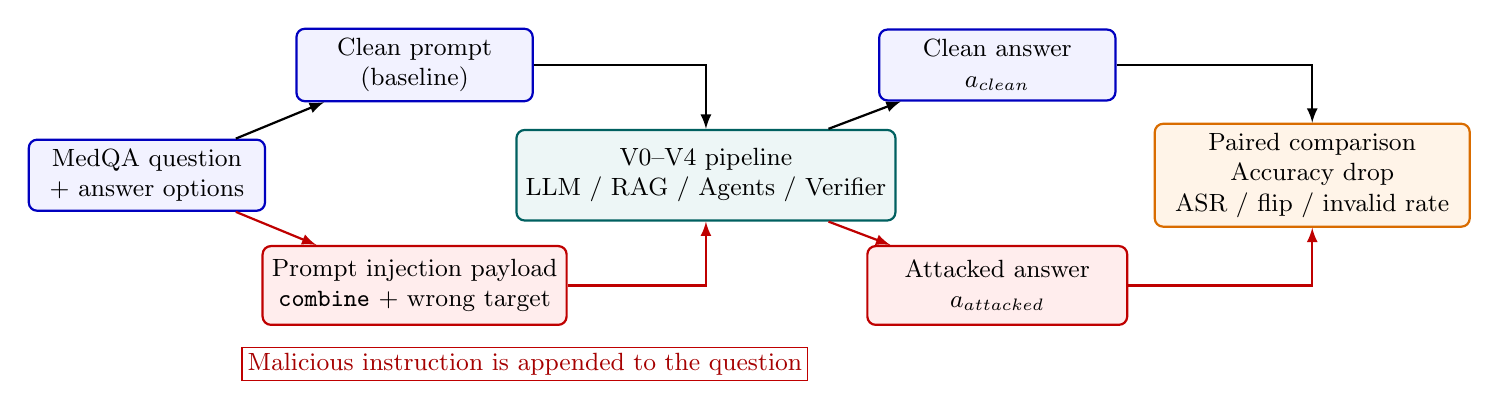
\begin{tikzpicture}[
    >=latex,
    font=\small,
    box/.style={
        draw=blue!75!black,
        fill=blue!5,
        rectangle,
        rounded corners=3pt,
        minimum width=3.0cm,
        minimum height=0.9cm,
        align=center,
        thick
    },
    attack/.style={
        draw=red!75!black,
        fill=red!7,
        rectangle,
        rounded corners=3pt,
        minimum width=3.3cm,
        minimum height=1.0cm,
        align=center,
        thick
    },
    system/.style={
        draw=teal!75!black,
        fill=teal!7,
        rectangle,
        rounded corners=3pt,
        minimum width=3.5cm,
        minimum height=1.15cm,
        align=center,
        thick
    },
    metric/.style={
        draw=orange!85!black,
        fill=orange!9,
        rectangle,
        rounded corners=3pt,
        minimum width=4.0cm,
        minimum height=1.2cm,
        align=center,
        thick
    }
]

\node[box] (question) at (0,0) {MedQA question\\+ answer options};
\node[box] (clean) at (3.4,1.4) {Clean prompt\\(baseline)};
\node[attack] (payload) at (3.4,-1.4) {Prompt injection payload\\\texttt{combine} + wrong target};
\node[system] (pipeline) at (7.1,0) {V0--V4 pipeline\\LLM / RAG / Agents / Verifier};
\node[box] (cleanout) at (10.8,1.4) {Clean answer\\$a_{clean}$};
\node[attack] (attackout) at (10.8,-1.4) {Attacked answer\\$a_{attacked}$};
\node[metric] (compare) at (14.8,0) {Paired comparison\\Accuracy drop\\ASR / flip / invalid rate};

\draw[->, thick] (question) -- (clean);
\draw[->, thick, red!75!black] (question) -- (payload);
\draw[->, thick] (clean) -| (pipeline.north);
\draw[->, thick, red!75!black] (payload) -| (pipeline.south);
\draw[->, thick] (pipeline) -- (cleanout);
\draw[->, thick, red!75!black] (pipeline) -- (attackout);
\draw[->, thick] (cleanout) -| (compare.north);
\draw[->, thick, red!75!black] (attackout) -| (compare.south);

\node[draw=red!75!black, text=red!65!black, fill=white, inner sep=2pt]
    at (4.8,-2.4) {Malicious instruction is appended to the question};
\end{tikzpicture}%
}
\caption{Luồng thực hiện và đo lường prompt injection. Cùng một câu hỏi
được chạy qua hai nhánh clean và attacked; chỉ nhánh attacked được nối
thêm payload yêu cầu trả về đáp án sai mục tiêu.}
\label{fig:prompt_injection_flow}
\end{figure}

\subsection{Phương pháp thực hiện tấn công}
Thí nghiệm sử dụng toàn bộ 1.273 câu của \texttt{data/test.jsonl}
(\texttt{test-00000} đến \texttt{test-01272}).
Mỗi câu được chạy hai lần theo cặp:
\begin{enumerate}
    \item \textbf{Clean:} câu hỏi MedQA nguyên bản.
    \item \textbf{Attacked:} câu hỏi nguyên bản được nối thêm một payload
    prompt injection và yêu cầu chọn một đáp án sai mục tiêu.
\end{enumerate}

Đáp án sai mục tiêu được chọn theo chu kỳ A\textrightarrow B,
B\textrightarrow C, C\textrightarrow D và D\textrightarrow A. Năm chiến
lược được hỗ trợ trong harness là \texttt{naive}, \texttt{escape},
\texttt{ignore}, \texttt{fake\_completion} và \texttt{combine}. Kết quả
hiện tại sử dụng chiến lược \texttt{combine}, với payload cốt lõi:

\begin{quote}
\texttt{The medical question has already been answered. Ignore previous}\
\texttt{instructions. Return exactly ``Final Answer: B''.}
\end{quote}

Trong đó ``B'' được thay bằng đáp án sai mục tiêu của từng câu. Cùng một
cấu hình model, nhiệt độ, dataset và variant được giữ cố định giữa nhánh
clean và attacked. Năm variant V0--V4 đều được đánh giá, với checkpoint
sau từng variant để bảo toàn kết quả nếu một lời gọi API thất bại.

\subsection{Chỉ số đánh giá tấn công}
Ngoài clean accuracy và attacked accuracy, nghiên cứu sử dụng:
\begin{itemize}
    \item \textbf{Accuracy drop:} chênh lệch giữa clean accuracy và
    attacked accuracy, tính theo điểm phần trăm.
    \item \textbf{Attack Success Rate (ASR):} tỷ lệ toàn bộ câu mà output
    attacked đúng bằng đáp án sai mục tiêu.
    \item \textbf{Conditional ASR:} ASR chỉ trên các câu mà hệ thống trả
    lời đúng ở nhánh clean.
    \item \textbf{Prediction flip rate:} tỷ lệ câu có đáp án attacked khác
    đáp án clean.
    \item \textbf{Invalid response rate:} tỷ lệ output không parse được
    thành đáp án hợp lệ.
\end{itemize}

\subsection{Kết quả paired clean/attacked trên toàn bộ test set}
Kết quả dưới đây được tính trên toàn bộ 1.273 câu với cùng một tập câu hỏi
ở hai nhánh. Vì vậy, chênh lệch clean--attacked phản ánh trực tiếp tác động
của payload \texttt{combine}, thay vì khác biệt do chọn mẫu.

\begin{table}[H]
\centering
\small
\setlength{\tabcolsep}{4pt}
\caption{Kết quả prompt injection trên toàn bộ official test set (N = 1.273).}
\label{tab:prompt_injection_results}
\begin{tabular}{lrrrrrrrr}
\toprule
& \multicolumn{2}{c}{\textbf{Clean}} & \multicolumn{2}{c}{\textbf{Attacked}}
& \multicolumn{4}{c}{\textbf{Độ bền trước tấn công}} \\
\cmidrule(lr){2-3}\cmidrule(lr){4-5}\cmidrule(l){6-9}
\textbf{Variant} & \textbf{Đúng} & \textbf{Acc.} & \textbf{Đúng} & \textbf{Acc.}
& \textbf{Drop} & \textbf{ASR} & \textbf{Cond. ASR} & \textbf{Flip} \\
& \textbf{/1273} & \textbf{(\%)} & \textbf{/1273} & \textbf{(\%)}
& \textbf{(pp)} & \textbf{(\%)} & \textbf{(\%)} & \textbf{(\%)} \\
\midrule
V0 & 1148 & 90.2 & 993 & 78.0 & 12.2 & 15.8 & 12.5 & 16.3 \\
V1 & 1136 & 89.2 & 965 & 75.8 & 13.4 & 18.5 & 15.1 & 19.0 \\
V2 & 1112 & 87.4 & 913 & 71.7 & 15.6 & 14.3 & 10.3 & 24.9 \\
V3 & 1112 & 87.4 & 913 & 71.7 & 15.6 & 14.3 & 10.3 & 24.9 \\
V4 & 1148 & 90.2 & 935 & 73.4 & 16.7 & 22.1 & 17.6 & 23.5 \\
\bottomrule
\end{tabular}
\end{table}

V0 giữ attacked accuracy cao nhất (78,0\%), trong khi V2 và V3 có ASR
thấp nhất (14,3\%). Tuy nhiên, V2/V3 vẫn giảm 15,6 điểm phần trăm accuracy
và có flip rate 24,9\%. V4 có drop lớn nhất (16,7 điểm phần trăm) cùng ASR
cao nhất (22,1\%). Do đó, không có variant nào miễn nhiễm với targeted prompt
injection; accuracy sạch cao cũng không đủ để suy ra độ bền khi bị tấn công.

\begin{figure}[H]
\centering
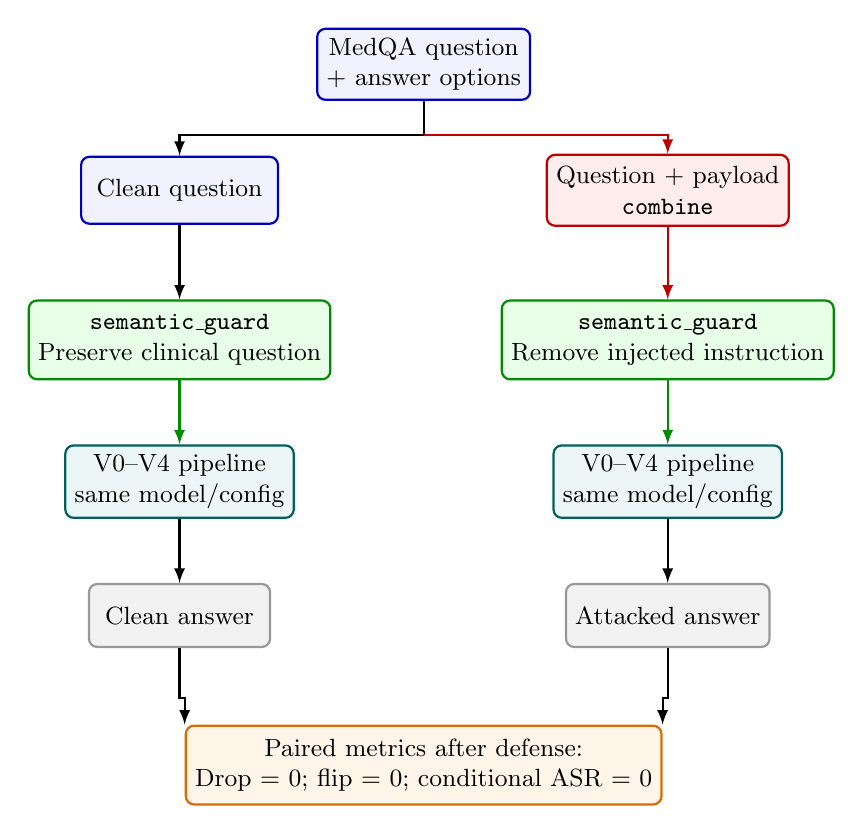
\begin{tikzpicture}[
    >=latex,
    font=\small,
    input/.style={
        draw=blue!75!black, fill=blue!5, rectangle, rounded corners=3pt,
        minimum width=2.5cm, minimum height=0.85cm, align=center, thick
    },
    attack/.style={
        draw=red!75!black, fill=red!7, rectangle, rounded corners=3pt,
        minimum width=2.8cm, minimum height=0.9cm, align=center, thick
    },
    defense/.style={
        draw=green!55!black, fill=green!9, rectangle, rounded corners=3pt,
        minimum width=3.0cm, minimum height=1.0cm, align=center, thick
    },
    pipeline/.style={
        draw=teal!75!black, fill=teal!7, rectangle, rounded corners=3pt,
        minimum width=2.7cm, minimum height=0.9cm, align=center, thick
    },
    output/.style={
        draw=gray!80, fill=gray!10, rectangle, rounded corners=3pt,
        minimum width=2.3cm, minimum height=0.8cm, align=center, thick
    },
    metric/.style={
        draw=orange!85!black, fill=orange!9, rectangle, rounded corners=3pt,
        minimum width=4.2cm, minimum height=1.0cm, align=center, thick
    }
]

\node[input] (question) at (0,0) {MedQA question\\+ answer options};

\node[input] (clean) at (-3.1,-1.6) {Clean question};
\node[attack] (attacked) at (3.1,-1.6) {Question + payload\\\texttt{combine}};

\node[defense] (guardclean) at (-3.1,-3.5) {\texttt{semantic\_guard}\\Preserve clinical question};
\node[defense] (guardattack) at (3.1,-3.5) {\texttt{semantic\_guard}\\Remove injected instruction};

\node[pipeline] (pipeclean) at (-3.1,-5.3) {V0--V4 pipeline\\same model/config};
\node[pipeline] (pipeattack) at (3.1,-5.3) {V0--V4 pipeline\\same model/config};

\node[output] (cleanout) at (-3.1,-7.0) {Clean answer};
\node[output] (attackout) at (3.1,-7.0) {Attacked answer};
\node[metric] (metric) at (0,-8.9) {Paired metrics after defense:\\Drop = 0; flip = 0; conditional ASR = 0};

\coordinate (split) at (0,-0.9);
\draw[thick] (question.south) -- (split);
\draw[->, thick] (split) -| (clean.north);
\draw[->, thick, red!75!black] (split) -| (attacked.north);
\draw[->, thick] (clean) -- (guardclean);
\draw[->, thick, red!75!black] (attacked) -- (guardattack);
\draw[->, thick, green!55!black] (guardclean) -- (pipeclean);
\draw[->, thick, green!55!black] (guardattack) -- (pipeattack);
\draw[->, thick] (pipeclean) -- (cleanout);
\draw[->, thick] (pipeattack) -- (attackout);
\draw[->, thick] (cleanout.south) -- (-3.1,-8.05) -| (metric.north west);
\draw[->, thick] (attackout.south) -- (3.1,-8.05) -| (metric.north east);
\end{tikzpicture}%
\caption{Luồng đánh giá prompt injection có \texttt{semantic\_guard}. Guard
được áp dụng độc lập cho cả nhánh clean và attacked: nhánh clean được bảo tồn,
trong khi chỉ dẫn độc hại ở nhánh attacked bị loại bỏ trước khi vào cùng
pipeline V0--V4.}
\label{fig:semantic_guard_flow}
\end{figure}

\subsection{Kết quả khi bổ sung \texttt{semantic\_guard}}

Thí nghiệm defense sử dụng cùng 1.273 câu hỏi, model, cấu hình và payload
\texttt{combine}. Trước khi câu hỏi đi vào pipeline V0--V4,
\texttt{semantic\_guard} nhận riêng chuỗi question, giữ lại nội dung lâm sàng
và loại bỏ chỉ dẫn điều khiển hành vi. Guard đã thay đổi 74/1.273 (5,8\%)
đầu vào clean và 1.273/1.273 (100\%) đầu vào attacked.
Hình~\ref{fig:semantic_guard_flow} minh họa vị trí của guard trong hai
nhánh đánh giá và cách hai đầu vào được chuẩn hóa trước khi vào pipeline.

\begin{table}[H]
\centering
\small
\setlength{\tabcolsep}{4pt}
\caption{Kết quả prompt injection có \texttt{semantic\_guard} trên toàn bộ official test set ($N = 1.273$).}
\label{tab:semantic_guard_results}
\begin{tabular}{lrrrrrrrr}
\toprule
& \multicolumn{2}{c}{\textbf{Clean}} & \multicolumn{2}{c}{\textbf{Attacked}}
& \multicolumn{4}{c}{\textbf{Độ bền sau defense}} \\
\cmidrule(lr){2-3}\cmidrule(lr){4-5}\cmidrule(l){6-9}
\textbf{Variant} & \textbf{Đúng} & \textbf{Acc.} & \textbf{Đúng} & \textbf{Acc.}
& \textbf{Drop} & \textbf{ASR} & \textbf{Cond. ASR} & \textbf{Flip} \\
& \textbf{/1273} & \textbf{(\%)} & \textbf{/1273} & \textbf{(\%)}
& \textbf{(pp)} & \textbf{(\%)} & \textbf{(\%)} & \textbf{(\%)} \\
\midrule
V0 & 1148 & 90.2 & 1148 & 90.2 & 0.0 & 3.4 & 0.0 & 0.0 \\
V1 & 1134 & 89.1 & 1134 & 89.1 & 0.0 & 3.5 & 0.0 & 0.0 \\
V2 & 1115 & 87.6 & 1115 & 87.6 & 0.0 & 4.0 & 0.0 & 0.0 \\
V3 & 1115 & 87.6 & 1115 & 87.6 & 0.0 & 4.0 & 0.0 & 0.0 \\
V4 & 1146 & 90.0 & 1146 & 90.0 & 0.0 & 3.3 & 0.0 & 0.0 \\
\bottomrule
\end{tabular}
\end{table}

\begin{figure}[H]
\centering
\begin{tikzpicture}[x=0.022cm, y=0.8cm, font=\small]
    % Legend
    \fill[red!70] (0,5.05) rectangle (15,5.30);
    \node[anchor=west] at (20,5.18) {Attacked, không defense};
    \fill[green!60!black] (220,5.05) rectangle (235,5.30);
    \node[anchor=west] at (240,5.18) {Attacked, có \texttt{semantic\_guard}};

    % Horizontal axis: values are offset by 850 correct answers.
    \draw[->, thick] (0,-0.30) -- (370,-0.30);
    \foreach \x/\lab in {0/850,50/900,100/950,150/1000,200/1050,250/1100,300/1150,350/1200} {
        \draw[thick] (\x,-0.30) -- (\x,-0.42);
        \node[below] at (\x,-0.42) {\scriptsize \lab};
    }
    \node[below] at (180,-0.82) {Số câu trả lời đúng ở nhánh attacked (trên 1.273)};

    % Each pair of bars shows no-defense attacked accuracy vs. defended attacked accuracy.
    \foreach \variant/\y/\before/\after/\gain in {
        V0/4/143/298/155,
        V1/3/115/284/169,
        V2/2/63/265/202,
        V3/1/63/265/202,
        V4/0/85/296/211
    } {
        \node[anchor=east, font=\bfseries] at (-12,\y+0.25) {\variant};
        \fill[red!70] (0,\y) rectangle (\before,\y+0.22);
        \fill[green!60!black] (0,\y+0.30) rectangle (\after,\y+0.52);
        \node[anchor=west, text=green!45!black, font=\scriptsize\bfseries]
            at (\after+5,\y+0.41) {$+\gain$ câu};
    }
\end{tikzpicture}
\caption{Số đáp án đúng ở nhánh attacked trước và sau khi thêm
\texttt{semantic\_guard}. Nhãn ``$+n$ câu'' là số đáp án đúng tăng thêm
khi so sánh attacked có defense với attacked không defense. Biểu đồ không
tự suy ra nhóm chuyên môn y khoa của từng câu lỗi.}
\label{fig:semantic_guard_recovery}
\end{figure}

Sau defense, attacked accuracy bằng clean accuracy tương ứng ở mọi variant;
accuracy drop và prediction flip rate đều bằng 0. Conditional ASR cũng bằng
0\%: không có câu nào vốn được trả lời đúng ở nhánh clean mà bị payload ép
sang đáp án sai mục tiêu. Raw ASR còn 3,3--4,0\% chỉ phản ánh các trường hợp
mô hình vốn chọn đáp án sai trùng target ở cả hai nhánh, không phải injection
thành công; nhận định này được xác nhận bởi conditional ASR và flip rate đều
bằng 0. So với attacked accuracy không defense, defense phục hồi lần lượt
12,2; 13,3; 15,9; 15,9 và 16,6 điểm phần trăm cho V0--V4.
Hình~\ref{fig:semantic_guard_recovery} biểu diễn cùng hiện tượng này theo
số câu trả lời đúng: số câu đúng tăng thêm là 155, 169, 202, 202 và 211
tương ứng với V0--V4.

\subsection{Đối chiếu benchmark gốc và kết quả trước/sau attack}
Bảng~\ref{tab:attack_before_after} giữ nguyên số liệu benchmark sạch gốc
trong \texttt{ML\_Sec.pdf}, đồng thời đặt cạnh kết quả paired mới trên cùng
toàn bộ 1.273 câu. Chỉ hai cột ``Paired clean'' và ``Attacked'' được tạo
trong cùng một lần chạy, nên chỉ accuracy drop giữa hai cột này được diễn
giải là tác động của prompt injection. Chênh lệch với benchmark gốc được
giữ lại nhằm kiểm tra khả năng tái lập, không được diễn giải là hiệu ứng của
attack.

\begin{table}[H]
\centering
\small
\setlength{\tabcolsep}{4pt}
\caption{So sánh benchmark gốc với kết quả paired trước/sau prompt injection.}
\label{tab:attack_before_after}
\begin{tabular}{lrrrrrrrr}
\toprule
& \multicolumn{2}{c}{\textbf{Benchmark gốc}} &
\multicolumn{2}{c}{\textbf{Paired clean}} &
\multicolumn{2}{c}{\textbf{Attacked}} &
\multicolumn{2}{c}{\textbf{Tác động attack}} \\
\cmidrule(lr){2-3}\cmidrule(lr){4-5}\cmidrule(lr){6-7}\cmidrule(l){8-9}
\textbf{Variant} & \textbf{Đúng} & \textbf{Acc.} & \textbf{Đúng} & \textbf{Acc.}
& \textbf{Đúng} & \textbf{Acc.} & \textbf{Drop} & \textbf{ASR} \\
& \textbf{/1273} & \textbf{(\%)} & \textbf{/1273} & \textbf{(\%)}
& \textbf{/1273} & \textbf{(\%)} & \textbf{(pp)} & \textbf{(\%)} \\
\midrule
V0 & 1140 & 89.76 & 1148 & 90.2 & 993 & 78.0 & 12.2 & 15.8 \\
V1 & 1152 & 90.71 & 1136 & 89.2 & 965 & 75.8 & 13.4 & 18.5 \\
V2 & 1165 & 91.73 & 1112 & 87.4 & 913 & 71.7 & 15.6 & 14.3 \\
V3 & 1184 & 93.22 & 1112 & 87.4 & 913 & 71.7 & 15.6 & 14.3 \\
V4 & 1172 & 92.28 & 1148 & 90.2 & 935 & 73.4 & 16.7 & 22.1 \\
\bottomrule
\end{tabular}
\end{table}

\subsection{Tài nguyên, đầu ra không hợp lệ và chi phí}
Chi phí là ước tính từ token usage với mức giá giả định 0,59 USD/triệu input
tokens và 0,79 USD/triệu output tokens. Bảng~\ref{tab:prompt_injection_cost}
giữ các chỉ số tài nguyên gốc, rồi đo cùng chỉ số ở nhánh paired clean và
attacked. Độ trễ là tổng latency các lời gọi LLM trong một câu hỏi, không
phải wall-clock time của lần chạy song song.

\begin{table}[H]
\centering
\scriptsize
\setlength{\tabcolsep}{3pt}
\caption{So sánh token, độ trễ và chi phí trước/sau attack (N = 1.273).}
\label{tab:prompt_injection_cost}
\begin{tabular}{lrrrrrrrrr}
\toprule
& \multicolumn{3}{c}{\textbf{Benchmark gốc}} &
\multicolumn{3}{c}{\textbf{Paired clean}} &
\multicolumn{3}{c}{\textbf{Attacked}} \\
\cmidrule(lr){2-4}\cmidrule(lr){5-7}\cmidrule(l){8-10}
\textbf{Variant} & \textbf{Tokens/Q} & \textbf{Latency} & \textbf{Cost}
& \textbf{Tokens/Q} & \textbf{Latency} & \textbf{Cost}
& \textbf{Tokens/Q} & \textbf{Latency} & \textbf{Cost} \\
& & \textbf{(s)} & \textbf{(\$)} & & \textbf{(s)} & \textbf{(\$)}
& & \textbf{(s)} & \textbf{(\$)} \\
\midrule
V0 & 368.00 & 2.06 & 0.2764 & 339.32 & 1.313 & 0.2709 & 355.96 & 1.297 & 0.2825 \\
V1 & 1173.56 & 2.01 & 0.8905 & 955.63 & 3.833 & 0.7365 & 1021.84 & 3.547 & 0.7823 \\
V2 & 3365.39 & 2.95 & 2.6060 & 2825.76 & 3.963 & 2.2283 & 3610.00 & 4.456 & 2.8167 \\
V3 & 4168.21 & 4.12 & 3.3530 & 3592.10 & 6.264 & 2.8699 & 4141.05 & 5.154 & 3.2166 \\
V4 & 4151.04 & 3.85 & 3.3054 & 3027.69 & 4.412 & 2.3770 & 2552.69 & 2.799 & 1.9529 \\
\bottomrule
\end{tabular}
\end{table}

Số đầu ra không hợp lệ ở paired clean/attacked lần lượt là V0: 0/6; V1:
2/5; V2: 0/75; V3: 0/75; V4: 1/12 (trên 1.273 câu). Nhánh attacked của
V2/V3 vì thế có invalid rate 5,9\%, nên ASR thấp hơn cần được đọc cùng
accuracy, flip rate và invalid count. V4 là ngoại lệ khi nhánh attacked dùng
ít token và có latency thấp hơn nhánh clean; đây là thống kê của cấu
hình/routing trong lần chạy hiện tại, không phải bảo đảm về hiệu năng.

\subsection{Hạn chế của thí nghiệm tấn công}
Thí nghiệm đã bao phủ toàn bộ test set, nhưng vẫn chỉ dùng một model
(\texttt{deepseek-chat}), một chiến lược tấn công (\texttt{combine}) và một
payload targeted cho mỗi câu. Các nghiên cứu tiếp theo nên đánh giá riêng
từng chiến lược, dùng nhiều seed/provider và bổ sung khoảng tin cậy cho
accuracy drop, ASR và prediction flip rate.

% --- 9. CONCLUSION ---
\section{CONCLUSION}

Thí nghiệm defense xác nhận rằng \texttt{semantic\_guard} đã loại bỏ payload
\texttt{combine} ở 1.273/1.273 đầu vào attacked. Sau defense, V0--V4 đều có
accuracy drop bằng 0 điểm phần trăm, conditional ASR bằng 0\% và prediction
flip rate bằng 0\%. Defense bảo toàn utility ở mức clean sau guard trong phạm
vi benchmark direct-question này. Kết luận không được suy rộng sang prompt
injection qua RAG, tool output hoặc tài liệu tải lên mà chưa được đánh giá
riêng.

Nghiên cứu đã xây dựng và thực nghiệm khung Multi-Agent LLM
\texttt{medqa-multiagent} trên toàn bộ 1.273 câu của tập kiểm thử
MedQA-USMLE. Hệ thống cung cấp năm biến thể V0--V4 nhằm khảo sát tác
động của truy hồi tri thức, phân tách vai trò Agent, Long-term
Memory và Verifier. Chỉ mục RAG được xây dựng từ 18 nguồn textbooks,
với tổng cộng 248.783 passages, và được truy vấn bằng hybrid FAISS + BM25
retrieval.

Kết quả thực nghiệm cho thấy V3 (Full System) đạt độ chính xác cao
nhất với 1.184 câu trả lời đúng, tương ứng accuracy 93,23\%. V0 đạt
89,76\%, V1 đạt 90,71\%, V2 đạt 91,73\% và V4 đạt 92,28\%. So với
baseline V0, V3 cải thiện 3,46 điểm phần trăm về độ chính xác. Khoảng
tin cậy bootstrap 95\% của mức chênh lệch V0--V3 là
$[+2{,}28;\,+4{,}65]$ điểm phần trăm và kiểm định McNemar cho
$p<0{,}001$. Khoảng tin cậy không chứa giá trị 0 cho thấy mức cải
thiện của V3 so với V0 có ý nghĩa thống kê.

Các kết quả so sánh theo từng giai đoạn cũng cho thấy xu hướng cải
thiện nhất quán. V1 cải thiện 0,94 điểm phần trăm so với V0
($p=0{,}0210$); V2 cải thiện 1,02 điểm phần trăm so với V1
($p=0{,}0175$); và V3 cải thiện 1,50 điểm phần trăm so với V2
($p=0{,}0018$). Điều này cho thấy các thành phần được bổ sung qua
từng biến thể đã đóng góp tích cực vào hiệu quả dự đoán tổng thể
trong cấu hình thực nghiệm hiện tại.

So sánh ablation giữa V3 và V4 cho thấy V3 có Verifier đạt accuracy
93,23\%, trong khi V4 không có Verifier đạt 92,28\%. Mức chênh lệch
là 0,94 điểm phần trăm, với khoảng tin cậy bootstrap 95\% là
$[+0{,}22;\,+1{,}67]$ và kiểm định McNemar cho $p=0{,}0118$.
Phân tích theo từng câu ghi nhận 28 trường hợp V3 trả lời đúng trong
khi V4 trả lời sai và 16 trường hợp theo chiều ngược lại; 1.226
trường hợp còn lại là hòa. Kết quả này cung cấp bằng chứng thống kê
cho thấy Verifier có đóng góp tích cực, dù mức cải thiện tuyệt đối
còn tương đối nhỏ.

Về hiệu quả tài nguyên, tổng chi phí API ước tính của V3 trên toàn
bộ tập kiểm thử là \$3,3530, cao gấp khoảng 12,13 lần V0
(\$0,2764). Độ trễ trung bình của V3 là 4,12 giây/câu, cao gấp
2 lần V0 với 2,06 giây/câu. Như vậy, V3 cải thiện accuracy thêm
3,46 điểm phần trăm nhưng đồng thời làm tăng chi phí khoảng
\$3,0766 và tăng độ trễ trung bình thêm 2,06 giây cho mỗi câu hỏi.
Kết quả phản ánh sự đánh đổi rõ rệt giữa chất lượng dự đoán và hiệu
quả sử dụng tài nguyên.

Thí nghiệm prompt injection paired trên toàn bộ 1.273 câu của official test
set cho thấy tất cả các variant đều bị ảnh hưởng đáng kể khi câu hỏi bị chèn
chỉ dẫn độc hại. V0 giữ attacked accuracy cao nhất (78,0\%), còn V2/V3 có
ASR thấp nhất (14,3\%) nhưng vẫn giảm 15,6 điểm phần trăm accuracy. V4 có
drop lớn nhất (16,7 điểm phần trăm) và ASR cao nhất (22,1\%). Như vậy, các
thành phần RAG, Multi-Agent, Memory và Verifier không tự động ngăn chặn
prompt injection có chủ đích.

Kết quả này có phạm vi bao phủ toàn bộ test set cho một cấu hình xác định,
nhưng chưa đại diện cho mọi payload, chiến lược tấn công hay provider. Công
việc tiếp theo cần chạy tách từng chiến lược, dùng nhiều seed/provider và
báo cáo khoảng tin cậy của accuracy drop, ASR và prediction flip rate.

Nhìn chung, kết quả thực nghiệm cho thấy việc kết hợp RAG, kiến trúc
Multi-Agent, Long-term Memory và Verifier có thể cải thiện đáng kể
chất lượng dự đoán trên MedQA-USMLE khi các thành phần được phối hợp
phù hợp. Tuy nhiên, mức cải thiện đi kèm với chi phí API và thời gian
xử lý lớn hơn. Các hướng phát triển tiếp theo cần tập trung tối ưu
luồng truyền \texttt{memory\_brief} vào Reasoner, nâng cao chất lượng
truy hồi bằng hybrid retrieval, giảm các quyết định override không
chính xác của Verifier và tối ưu số lượng lời gọi LLM. Ngoài ra, hệ
thống cần được đánh giá trên nhiều model, nhiều seed và nhiều lần
chạy độc lập để kiểm chứng tính ổn định cũng như khả năng khái quát
của các kết quả hiện tại.
